\section{La integral definida}

\textbf{Definició:} Donada una funció $f(x)$ contínua en un interval tancat $[a, b]$, s'anomena \textbf{integral definida} de $f(x)$ entre $a$ i $b$ el nombre

\begin{equation}
I = \int_a^b f(x)\,dx
\end{equation}

on $a$ és el límit inferior i $b$ és el límit superior d'integració.

Geomètricament, si $f(x) \ge 0$ a $[a, b]$, la integral definida representa l'àrea de la regió compresa entre la corba $y = f(x)$, l'eix $OX$ i les rectes verticals $x = a$ i $x = b$:

\begin{figure}[!htbp]
\centering
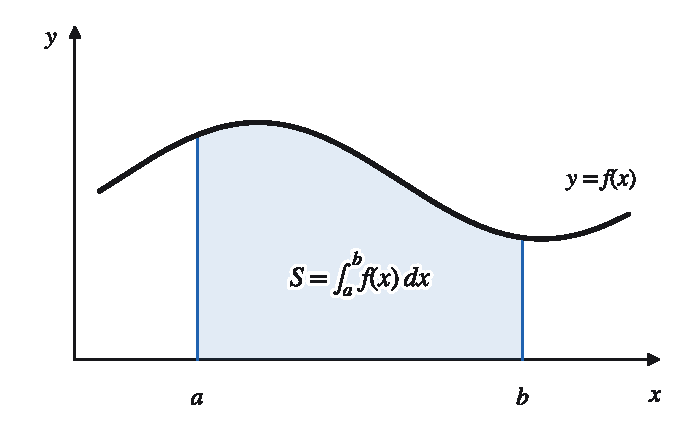
\includegraphics[width=330pt]{fig/m05_f12.pdf}
\caption{L'àrea $S$ sota la corba $f(x)$ entre $x = a$ i $x = b$ és igual a $\int_a^b f(x)\,dx$.}
\end{figure}

\section{La fórmula de Barrow. El càlcul integral}

\textbf{Propietat (Fórmula de Barrow):} Si $F(x)$ és una primitiva de $f(x)$ a $[a, b]$, aleshores

\begin{equation}
\int_a^b f(x)\,dx = \Bigl[F(x)\Bigr]_a^b = F(b) - F(a)
\end{equation}

La fórmula de Barrow connecta el càlcul de primitives (integral indefinida) amb el càlcul d'àrees (integral definida), i constitueix el \textbf{teorema fonamental del càlcul integral}.

\section{Càlcul d'àrees}

La integral definida és l'eina principal per calcular àrees de regions planes.

\subsection{Àrea compresa entre la gràfica d'una funció i l'eix OX}

Quan la funció talla l'eix $OX$ en punts intermedis $c_1, c_2, \dots$ dins de $[a, b]$, l'àrea total s'expressa com la suma del valor absolut de les integrals en cada subinterval:

\begin{equation*}
A = \left\lvert\int_a^{c_1} f(x)\,dx\right\rvert + \left\lvert\int_{c_1}^{c_2} f(x)\,dx\right\rvert + \left\lvert\int_{c_2}^{b} f(x)\,dx\right\rvert
\end{equation*}

\emph{Observació:} el valor absolut és necessari perquè la integral resulta negativa quan la funció és per sota de l'eix $OX$. Sense el valor absolut, les àrees positives i negatives es cancel\textperiodcentered{}larien parcialment.

\begin{figure}[!htbp]
\centering
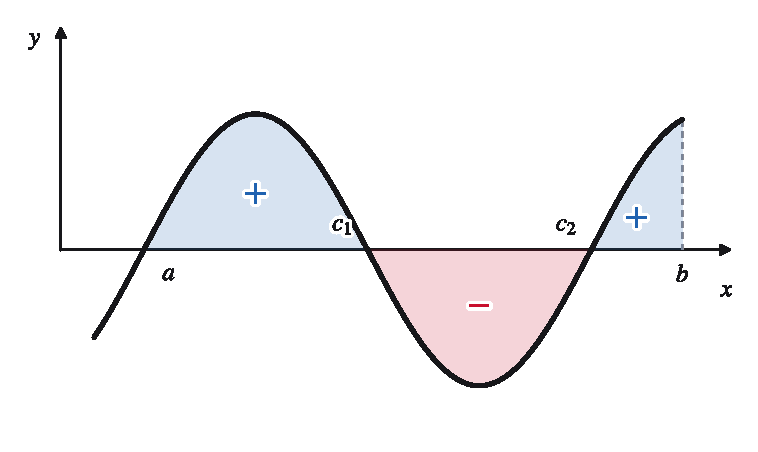
\includegraphics[width=364pt]{fig/m05_f13.pdf}
\caption{L'àrea total entre la corba i l'eix $OX$ és la suma dels valors absoluts de cada integral parcial. La zona negativa (funció per sota de l'eix) s'ha de prendre en valor absolut.}
\end{figure}

\subsection{Àrea compresa entre les gràfiques de dues funcions}

Per calcular l'àrea de la regió compresa entre dues corbes $f(x)$ i $g(x)$ en l'interval $[a, b]$:

\begin{enumerate}
\item Es troben els punts d'intersecció resolent $f(x) = g(x)$; aquests donen els límits d'integració.
\item Es calcula la diferència entre la funció superior i la inferior:
\end{enumerate}

\begin{equation*}
A = \int_a^b \bigl[g(x) - f(x)\bigr]\,dx
\end{equation*}

on $g(x) \ge f(x)$ a tot l'interval $[a, b]$.

\begin{figure}[!htbp]
\centering
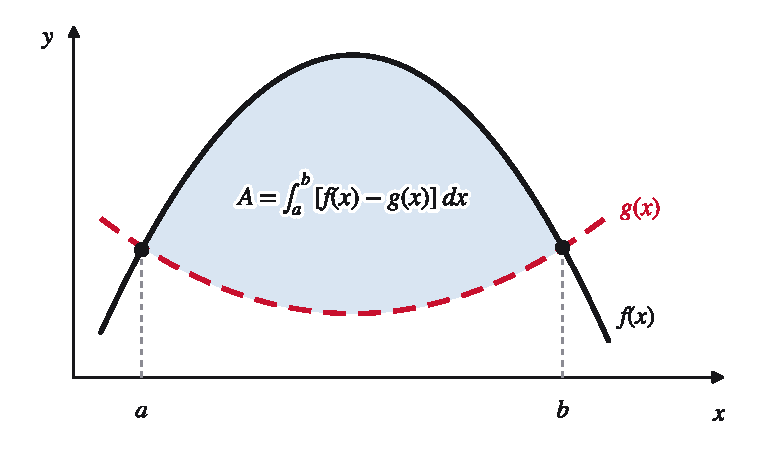
\includegraphics[width=364pt]{fig/m05_f13b.pdf}
\caption{Àrea entre les gràfiques de $f(x)$ i $g(x)$ en $[a, b]$.}
\end{figure}

\section{Complement: propietats de la integral definida}

Les propietats següents són vàlides sempre que les funcions siguin integrables als intervals indicats:

\begin{table}[!htbp]
\centering
\renewcommand{\arraystretch}{1.75}
\begin{tabular}{lc}
\toprule
Propietat & Expressió \\
\midrule
Interval degenerat & $\displaystyle \displaystyle\int_a^a f(x)\,dx = 0$ \\
Inversió dels límits & $\displaystyle \displaystyle\int_a^b f(x)\,dx = -\int_b^a f(x)\,dx$ \\
Linealitat (suma) & $\displaystyle \displaystyle\int_a^b [f(x) + g(x)]\,dx = \int_a^b f(x)\,dx + \int_a^b g(x)\,dx$ \\
Linealitat (escalar) & $\displaystyle \displaystyle\int_a^b k\,f(x)\,dx = k\int_a^b f(x)\,dx, \quad k \in \mathbb{R}$ \\
Additivitat en intervals & $\displaystyle \displaystyle\int_a^b f(x)\,dx = \int_a^c f(x)\,dx + \int_c^b f(x)\,dx, \quad a < c < b$ \\
Monotonia & Si $\displaystyle f(x) \le g(x)$ a $\displaystyle [a, b]$, llavors $\displaystyle \displaystyle\int_a^b f\,dx \le \int_a^b g\,dx$ \\
Fita de la integral & $\displaystyle \displaystyle\left\lvert\int_a^b f(x)\,dx\right\rvert \le \int_a^b |f(x)|\,dx$ \\
\bottomrule
\end{tabular}
\end{table}

\begin{figure}[!htbp]
\centering
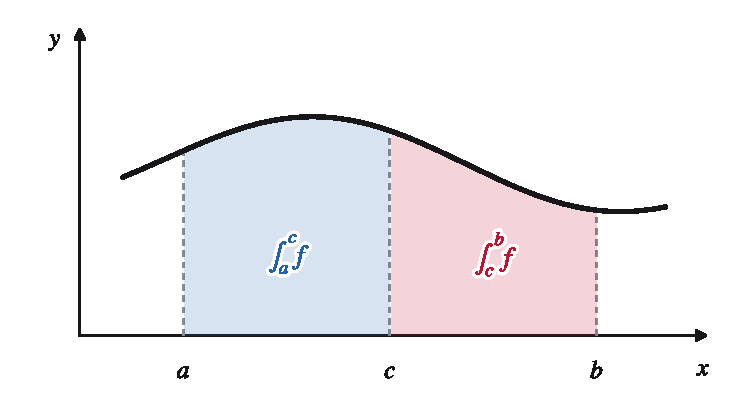
\includegraphics[width=353pt]{fig/m05_f25.pdf}
\caption{Propietat d'additivitat: $\int_a^b f = \int_a^c f + \int_c^b f$.}
\end{figure}

\section{Complement: teorema fonamental del càlcul}

\textbf{Teorema fonamental del càlcul:} si $f$ és contínua en $[a, b]$, la funció ``àrea acumulada''

\begin{equation}
F(x)=\int_a^x f(t)\,dt
\end{equation}

és derivable i $F'(x)=f(x)$ per a tot $x\in(a,b)$.

És a dir, \textbf{integrar i derivar són operacions inverses}. Si la variable apareix en un límit d'integració que és una funció $u(x)$, s'aplica la regla de la cadena:

\begin{equation*}
\frac{d}{dx}\int_a^{u(x)} f(t)\,dt=f\bigl(u(x)\bigr)\cdot u'(x)
\end{equation*}

\emph{Exemple 1:} Si $G(x)=\displaystyle\int_0^{x^2}\sin t\,dt$, llavors $G'(x)=\sin(x^2)\cdot 2x$.

\emph{Exemple 2 (amb límits):} $\displaystyle\lim_{x\to0}\frac{1}{x^2}\int_0^x\sin t\,dt$. És una indeterminació $\frac00$; per Hôpital, el numerador es deriva amb el teorema fonamental:

\begin{equation*}
\lim_{x\to0}\frac{\sin x}{2x}=\frac12
\end{equation*}

\emph{Exemple 3 (extrems):} Si $F(x)=\displaystyle\int_0^x (t^2-4)\,dt$, els punts crítics surten de $F'(x)=x^2-4=0$, és a dir, $x=\pm2$, sense calcular la integral.

\section{Complement: mètode per calcular àrees}

\subsection{Mètode}

\begin{enumerate}
\item \textbf{Fer un esquema} de les gràfiques (encara que sigui aproximat).
\item Trobar els \textbf{punts de tall} entre les corbes (o amb l'eix $OX$) resolent $f(x)=g(x)$: són els límits d'integració.
\item Veure \textbf{quina funció està per sobre} en cada tram. Si s'alternen, cal dividir en trams.
\item Calcular $\displaystyle S=\int_a^b\bigl(f_{\text{superior}}-f_{\text{inferior}}\bigr)\,dx$ en cada tram i sumar.
\item L'àrea és sempre \textbf{positiva}. \emph{Pregunta clàssica:} $\displaystyle\int_0^{2\pi}\sin x\,dx=0$, però l'àrea entre $\sin x$ i l'eix $OX$ en $[0,2\pi]$ és $2\displaystyle\int_0^{\pi}\sin x\,dx=4$.
\end{enumerate}

\subsection{Exemple 1 --- Entre una paràbola i una recta}

Àrea limitada per $f(x)=x^2$ i $g(x)=2x$.

\begin{itemize}
\item \textbf{Punts de tall:} $x^2=2x\Rightarrow x(x-2)=0\Rightarrow x=0,\ x=2$.
\item En $(0,2)$, per exemple $x=1$: $g(1)=2>f(1)=1$, així que la recta és la superior.
\end{itemize}

\begin{equation*}
S=\int_0^2\left(2x-x^2\right)dx=\left[x^2-\frac{x^3}{3}\right]_0^2=4-\frac83=\frac43\ \text{u}^2
\end{equation*}

\begin{figure}[!htbp]
\centering
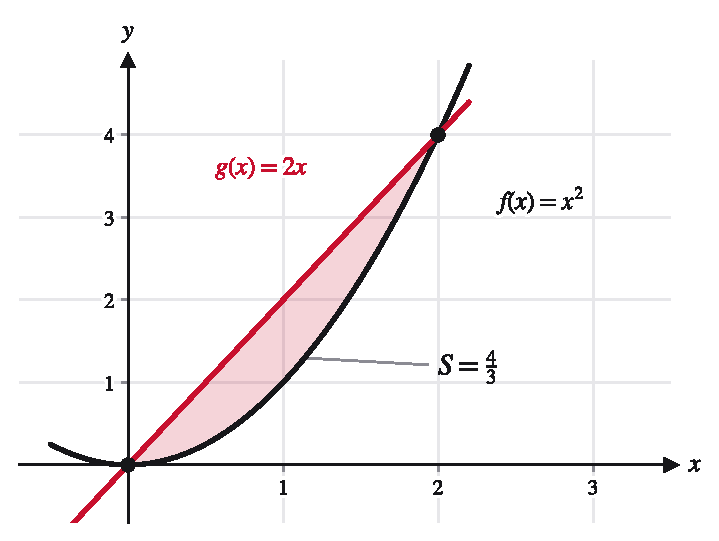
\includegraphics[width=345pt]{fig/m05_f35.pdf}
\caption{L'àrea tancada entre $f(x)=x^2$ i $g(x)=2x$ val $\frac43$.}
\end{figure}

\subsection{Exemple 2 --- Les gràfiques es creuen: $y=x^3$ i $y=x$}

\begin{itemize}
\item \textbf{Talls:} $x^3=x\Rightarrow x(x-1)(x+1)=0\Rightarrow x=-1,\,0,\,1$.
\item En $(-1,0)$: $x^3>x$ (per exemple, $x=-0{,}5$: $-0{,}125>-0{,}5$). En $(0,1)$: $x>x^3$.
\end{itemize}

\begin{equation*}
S_1=\int_{-1}^{0}(x^3-x)\,dx=\left[\frac{x^4}{4}-\frac{x^2}{2}\right]_{-1}^{0}=\frac14,\qquad S_2=\int_0^1(x-x^3)\,dx=\left[\frac{x^2}{2}-\frac{x^4}{4}\right]_0^1=\frac14
\end{equation*}

\begin{equation*}
S=S_1+S_2=\frac12\ \text{u}^2
\end{equation*}

\emph{Si es calculés $\int_{-1}^{1}(x-x^3)\,dx$ d'un sol cop, donaria $0$ per simetria: per això cal dividir en trams.}

\begin{figure}[!htbp]
\centering
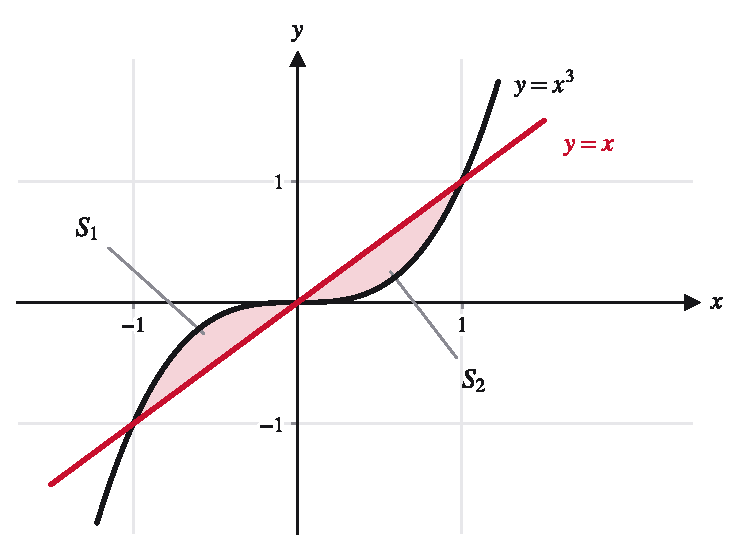
\includegraphics[width=356pt]{fig/m05_f36.pdf}
\caption{Àrea entre $y=x^3$ i $y=x$: dos trams iguals, $S_1$ i $S_2$, amb la funció superior diferent en cada un.}
\end{figure}

\section{Complement: demostracions del teorema fonamental i de la regla de Barrow}

\subsection{Teorema fonamental del càlcul}

\textbf{Teorema:} si $f$ és contínua en $[a,b]$, la funció $F(x)=\displaystyle\int_a^x f(t)\,dt$ és derivable i $F'(x)=f(x)$.

\emph{Demostració.} Per a $h>0$ petit, per la propietat d'additivitat de la integral,

\begin{equation*}
\frac{F(x+h)-F(x)}{h}=\frac1h\int_x^{x+h}f(t)\,dt
\end{equation*}

Com que $f$ és contínua en $[x,x+h]$, per Weierstrass té un mínim $m_h$ i un màxim $M_h$ en aquest interval, i l'àrea es pot acotar:

\begin{equation*}
m_h\le\frac1h\int_x^{x+h}f(t)\,dt\le M_h
\end{equation*}

Quan $h\to0$, per continuïtat, $m_h\to f(x)$ i $M_h\to f(x)$. Pel teorema de l'entrepà, el quocient tendeix a $f(x)$, és a dir, $F'(x)=f(x)$. (Per a $h<0$ es fa igual.) $\blacksquare$

\subsection{Regla de Barrow}

\textbf{Regla de Barrow:} si $f$ és contínua en $[a,b]$ i $G$ és una primitiva qualsevol de $f$, llavors

\begin{equation}
\int_a^b f(x)\,dx=G(b)-G(a)
\end{equation}

\emph{Demostració.} Siguin $F(x)=\int_a^x f$ i $G$ una primitiva. Com que $F'=f=G'$, la funció $F-G$ té derivada zero en tot l'interval i, per la conseqüència del teorema del valor mitjà, és constant: $F(x)=G(x)+C$.

Com que $F(a)=0$, resulta $C=-G(a)$. Llavors

\begin{equation*}
\int_a^b f(x)\,dx=F(b)=G(b)-G(a).\ \blacksquare
\end{equation*}

\textbf{Per què importa:} és el que permet calcular àrees amb primitives sense haver de fer límits de sumes de Riemann.

\section{Complement: sumes de Riemann i definició de la integral definida}

Per definir l'àrea sota una corba es divideix $[a,b]$ en $n$ subintervals i s'aproxima amb rectangles. La \textbf{suma inferior} $s_n$ usa el mínim de $f$ en cada subinterval i la \textbf{suma superior} $S_n$ el màxim.

\begin{figure}[!htbp]
\centering
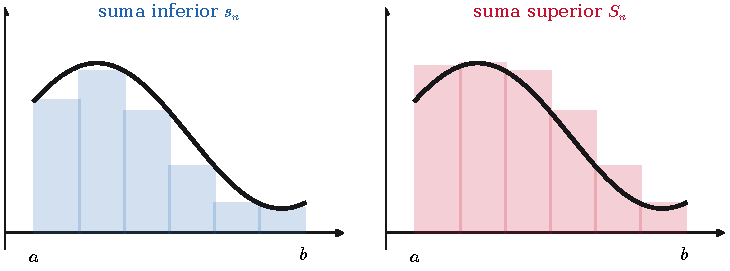
\includegraphics[width=350pt]{fig/x05_riemann.pdf}
\caption{Sumes de Riemann de $f$ en $[a,b]$ amb $n=6$ subintervals: la suma inferior $s_n$ (esquerra) i la superior $S_n$ (dreta) emmarquen l'àrea.}
\end{figure}

\textbf{Definició:} Si $f$ és contínua en $[a,b]$, les sumes inferiors i superiors tenen el mateix límit quan $n\to\infty$, i aquest límit és la \textbf{integral definida}:

\begin{equation}
\int_a^b f(x)\,dx=\lim_{n\to\infty}\sum_{i=1}^{n}f(x_i)\,\Delta x,\qquad\Delta x=\frac{b-a}{n}.
\end{equation}

\emph{Exemple:} Calculem $\displaystyle\int_0^1x^2dx$ pel límit de sumes. Amb $x_i=\dfrac in$ i $\Delta x=\dfrac1n$,

\begin{equation*}
\sum_{i=1}^{n}\frac{i^2}{n^2}\cdot\frac1n=\frac{1}{n^3}\cdot\frac{n(n+1)(2n+1)}{6}\xrightarrow[n\to\infty]{}\frac13.
\end{equation*}

El mateix resultat s'obté amb Barrow: $\left[\dfrac{x^3}{3}\right]_0^1=\dfrac13$.

\section{Complement: teorema del valor mitjà del càlcul integral}

\textbf{Teorema (del valor mitjà del càlcul integral):} Si $f$ és contínua en $[a,b]$, existeix almenys un punt $c\in[a,b]$ tal que

\begin{equation}
\int_a^b f(x)\,dx=f(c)\,(b-a).
\end{equation}

El nombre $f(c)=\dfrac{1}{b-a}\displaystyle\int_a^b f(x)\,dx$ s'anomena \textbf{valor mitjà} de $f$ en $[a,b]$: l'alçada d'un rectangle de base $b-a$ amb la mateixa àrea que la regió sota la corba.

\begin{figure}[!htbp]
\centering
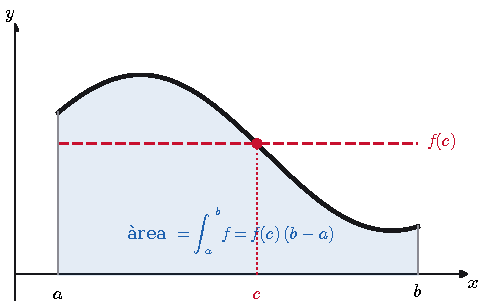
\includegraphics[width=233pt]{fig/x05_mean_value.pdf}
\caption{Teorema del valor mitjà del càlcul integral: l'àrea sota $f$ coincideix amb la del rectangle d'alçada $f(c)$ i base $b-a$.}
\end{figure}

\emph{Demostració.} Per Weierstrass, $f$ té mínim $m$ i màxim $M$ en $[a,b]$. Aleshores $m(b-a)\le\int_a^bf\le M(b-a)$, així que $\frac1{b-a}\int_a^bf$ és un valor entre $m$ i $M$; pel teorema dels valors intermedis, $f$ el pren en algun punt $c$. $\blacksquare$

\emph{Exemple:} Per a $f(x)=x^2$ en $[0,3]$: $\int_0^3x^2dx=9$, el valor mitjà és $\dfrac93=3$ i s'assoleix en $c=\sqrt3\approx1{,}73$.

\section{Complement: volum d'un cos de revolució}

Si la regió sota $y=f(x)$ entre $x=a$ i $x=b$ gira al voltant de l'eix $OX$, es genera un cos de revolució. Cada secció perpendicular a l'eix és un cercle de radi $f(x)$, amb àrea $\pi f(x)^2$; sumant-les s'obté

\begin{equation*}
V=\pi\int_a^b\bigl[f(x)\bigr]^2dx.
\end{equation*}

\begin{figure}[!htbp]
\centering
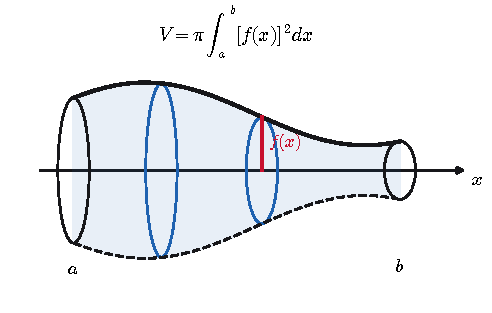
\includegraphics[width=236pt]{fig/x05_revolution.pdf}
\caption{Cos de revolució generat en girar $y=f(x)$ al voltant de l'eix $OX$: cada secció és un cercle de radi $f(x)$.}
\end{figure}

\emph{Exemples:} 

a) \emph{Con:} $y=x$ entre $0$ i $3$. $V=\pi\displaystyle\int_0^3x^2dx=\pi\cdot9=9\pi$ (coincideix amb $\frac13\pi r^2h$ per a $r=h=3$).

b) \emph{Paraboloide:} $y=\sqrt x$ entre $0$ i $4$. $V=\pi\displaystyle\int_0^4x\,dx=\pi\cdot8=8\pi$.

c) \emph{Esfera:} $y=\sqrt{r^2-x^2}$ entre $-r$ i $r$. $V=\pi\displaystyle\int_{-r}^{r}(r^2-x^2)\,dx=\pi\Bigl(2r^3-\dfrac{2r^3}{3}\Bigr)=\dfrac43\pi r^3$.

\section{Complement: més exemples d'àrees}

\emph{Exemple 1:} Àrea compresa entre $y=\sin x$ i l'eix $OX$ en $[0,2\pi]$. La funció canvia de signe en $x=\pi$, així que

\begin{equation*}
A=\int_0^{\pi}\sin x\,dx+\Bigl|\int_\pi^{2\pi}\sin x\,dx\Bigr|=2+|-2|=4.
\end{equation*}

(La integral sense separar donaria $0$: les àrees positiva i negativa es compensarien.)

\emph{Exemple 2:} Àrea entre $y=\sin x$ i $y=\cos x$ entre dues interseccions consecutives, $x=\frac\pi4$ i $x=\frac{5\pi}4$. En aquest interval $\sin x\ge\cos x$, per tant

\begin{equation*}
A=\int_{\pi/4}^{5\pi/4}(\sin x-\cos x)\,dx=\bigl[-\cos x-\sin x\bigr]_{\pi/4}^{5\pi/4}=\sqrt2+\sqrt2=2\sqrt2.
\end{equation*}

\emph{Exemple 3:} Àrea compresa entre $y=x^2$ i la recta $y=x+2$. Interseccions: $x^2=x+2\Rightarrow x=-1,\,2$. A $[-1,2]$ la recta està per sobre:

\begin{equation*}
A=\int_{-1}^{2}(x+2-x^2)\,dx=\Bigl[\frac{x^2}{2}+2x-\frac{x^3}{3}\Bigr]_{-1}^{2}=\frac{9}{2}.
\end{equation*}
